\section{\dtn}
\label{penning2019dtn7:sec:implementation}

In this section, we present the design and implementation of \dtn. 
%At first we identify the requirements for a DTN software. 
%On this basis we choose a programming language to match our goals and design interfaces and APIs for application software. 
%We then present an architectural overview on \dtn and the resulting daemon and application. 

\subsection{Requirements Analysis}
%For DTN software, which requires an installation in as many locations as possible for a functioning network, the factors of operating system and hardware independence as well as fast deployment play a major role. 
There are several requirements that should be satisfied by DTN software. First, DTN software operating on a variety of laptops, smartphones, and routers should run on several hardware architectures (e.g., x86, ARM, and MIPS), based on the most popular operating systems (e.g., Linux, macOS, and Windows).
Second, the individual components of the DTN software should be exchangeable.
For example, there is the need to support different storage backends, CLAs, and DTN routing protocols.
A suitable programming interface enabling concurrent execution is required for the interaction of components.  
Furthermore, a CLA implementation is required as well as a peer discovery mechanism to enable automatic establishment of connections between nodes.
Finally, applications should to be independent of the DTN software, to allow easy creation of further applications and tools.
Thus, a convenient interface between the DTN software and applications is required.



\subsection{Implementation Decisions}

As a result of these requirements, we selected the Go programming language\footnote{\url{https://golang.org}} to develop \dtn.
Go offers a large standard library and is rather developer-friendly.  Its strengths are the simple creation and integration of programming libraries. 
Moreover, Go enforces good style guides and clean code plus provides memory-safety guarantees to increase security and stability of written programs. Thus, Go makes maintaining code and bringing in new developers very easy.
The source code including all required dependencies are compiled into a single, static executable, removing the need for interpreters or further libraries.
Furthermore, the Go compiler allows simple (cross-)compilation for many operating systems and processor architectures.
The concept of concurrency is implemented in Go through the interaction of Goroutines and Channels; concurrency was one of the design priorities of the language designers. 
%Concluding, the Go programming language is a suitable programming platform for the development of a complete DTN software.


To support exchangeability of \dtn's components, we structured our implementation into \textit{Bundles} and its corresponding \textit{Store}, \textit{Convergence Layer Adapters}, \textit{Peer Discovery}, the \textit{Application Agent}, \textit{Routing}, and the \textit{Core} package needed to connect the individual packages.
The modules in the these packages are designed as generic interfaces and example implementations, e.g., there exists an interface for routing in general and an epidemic routing implementation.
We decided to use MTCP for exchanging messages between two \dtn nodes due to its simplicity. 
A third party application can also use parts of \dtn as a library to, e.g., create and serialize bundles via the corresponding package.
To make programming of applications against these interfaces simple and programming language independent, we decided to use a RESTful API.


\subsection{\dtn Architecture}
\begin{figure}[ht!]
    \centering
    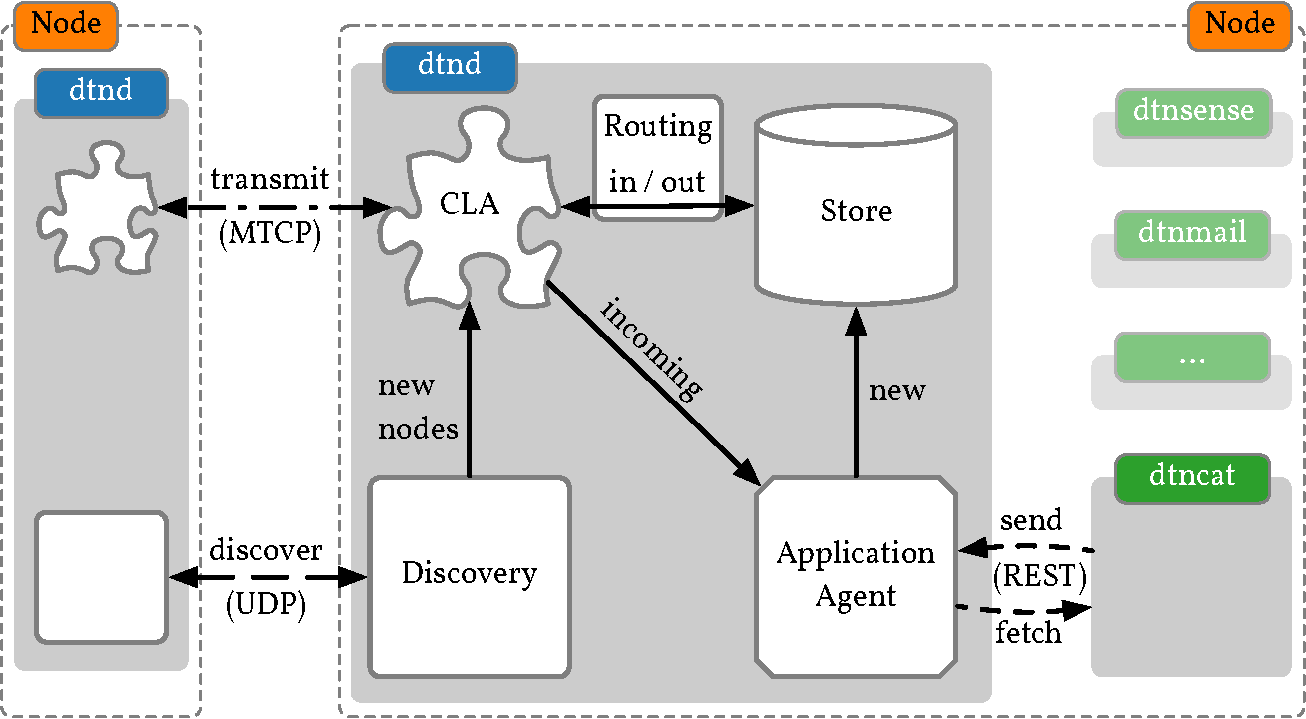
\includegraphics[width=0.9\columnwidth]{figs/application_overview.pdf}
    \caption{Architecture and data flow in \dtn}
    \label{penning2019dtn7:fig:overview}
\end{figure}

Fig.~\ref{penning2019dtn7:fig:overview} shows the modules of \dtn and their interaction.
The arrows indicate the way a bundle is internally processed in \dtn. 
The links between two distinct \dtn nodes are shown by both an active CLA and the Discovery on the figure's left hand side. 
Multiple client connections to the AA from within the node are delineated on the node's right hand side.

% Store
To store bundles locally, a serialized version as defined in BP7 is written to the file system. 
A central index of all known bundles manages their meta-data and links point to information of the specific file.
This index supports a fast lookup of bundles. The module providing this functionality is called \textit{Store}.

% AA, REST
In \dtn, an AA is implemented as a RESTful Web API to support both dispatching and fetching of bundles. 
The API does not interact with entire bundles, but only with a subset of its fields.
This allows a client to send a new bundle by only supplying the destination EID and a payload. 
Such a request can easily be created from the command line or possible third-party software.
When fetched over the API, selected fields of those bundles are returned and the bundles will be removed from the store afterwards.

% CLA
The concept of different CLs and their CLAs is also present in \dtn's architecture with an implementation of MTCP.
Based on a specific CL's characteristics, bundles might be transferred in a uni- or bidirectional way. Thus, a CLA in \dtn must supply one or multiple modules for inbound and outbound bundle processing.
The unidirectional MTCP is designed using modules for sending and receiving bundles.

% Discovery
To support connections in dynamic networks, a \textit{Peer Discovery} mechanism is provided. It announces a node's existence and listens for potential neighbors.
This discovery mechanism broadcasts all of the node's CLAs continuously and notifies about received CLAs.

% Core
The previously defined components are linked together within \dtn's \textit{Core} package. 
A central processing pipeline consumes both newly created and inbound bundles. 
Within this pipeline, a bundle will be marked to be delivered to a subset of known CLAs, to a local AA or to be discarded for later processing or even removed.
The Core's internal links, visualized in Fig.~\ref{penning2019dtn7:fig:overview}, are related to the concept of a BPA, and serve as an interface between CLAs and the AA.

%% Routing
Every bundle that is not addressed to a particular node will be forwarded over one or multiple CLAs to neighboring nodes.
The decision about which CLAs to select is made by a routing algorithm.
To support the use of different routing algorithms, a generic interface needs to be informed about inbound bundles and, furthermore, a tight cohesiveness to the core is required.
\dtn implements an epidemic routing module, which is notified about received bundles, to memorize both sender and receiver.
Before dispatching, the epidemic routing algorithm compiles a subset of known connections which have not received this bundle yet.

% Library
Finally, \dtn is also intended to be used as a library and allows fast development of DTN applications. In particular, bundle package creation, serialization, and deserialization  might be useful in other software.


\subsection{Resulting Programs}

\dtn contains a DTN daemon, referred to as \texttt{dtnd} in Fig.~\ref{penning2019dtn7:fig:overview}, for storing and exchanging bundles and interfacing with applications. Currently, an example DTN application (\texttt{dtncat} in Fig.~\ref{penning2019dtn7:fig:overview}) for sending and receiving bundles, implemented as a command line tool, is included. 
\texttt{dtnd} initializes the previously defined modules according to the configuration provided by the user.
\texttt{dtncat} processes user input, which is handed over to \texttt{dtnd}'s AA RESTful interface.
The input is then encapsulated inside the Payload Block of a newly created bundle by \texttt{dtnd}. This bundle's Primary Block will be populated with basic defaults, like disabled CRC, and a delivery report request.
As shown in Listing~\ref{penning2019dtn7:lst:dtncat}, \texttt{dtncat} is called by passing parameters on the command line. 
The first option selects between receiving or sending bundles.
The local \texttt{dtnd}, running the RESTful API, is addressed by the second parameter. 
When sending new bundles, the content is read from the standard input.

\begin{lstlisting}[caption={\texttt{dtncat} example}, captionpos={b}, label={penning2019dtn7:lst:dtncat}]
# Sending a bundle
$ dtncat send http://localhost:8080 dtn:s2 <<< "3782 lx"

# Retrieving a received bundle 
$ dtncat fetch http://localhost:8080 
\end{lstlisting}

